\documentclass{article}
\usepackage[utf8]{inputenc}
\usepackage{url}
\usepackage{graphicx}
\usepackage{float}
\usepackage{array}
\usepackage[export]{adjustbox}

\usepackage{todonotes}
\usepackage{bytefield}


\usepackage{enumitem}

\newlist{registerdescription}{description}{2}
\setlist[registerdescription]{labelwidth=1.5cm,leftmargin=!,font=\normalfont}

\usepackage{geometry}
 \geometry{
   a4paper,
   total={170mm,257mm},
   left=30mm,
   right=30mm,
   top=15mm,
 }

\title{Embedded systems Laboratoy 3 \\
        Design of an Avalon camera controller}
\author{
  Snoeijs, Jan\\
  EPFL\\
  \texttt{jan.snoeijs@epfl.ch}
  \and
  Spieler, Michael\\
  EPFL\\
  \texttt{spieler.micheal@epfl.ch}
  }
\date{November 2017}

\begin{document}

\maketitle

\section{Introduction}

For this lab work we chose to design the component for the Terasic THDB-D5M camera. In this document we detail the complete design of the component and explain the synchronization between our component and an Avalon interfaced LCD controller. We will also present how the NIOS II processor should be programmed to control the hardware component and handle the synchronization between camera and LCD.

\section{Camera controller overview}

In this section we present the system architecture and how it is divided in the different sub-components and their interaction.

\subsection{High-level architecture}
Figure \ref{fig:full_system} illustrates the full system architecture view. A NIOS-II processor runs with data and code form the internal SRAM memory. The Camera is connected to our custom camera controller. The camera controller is configured through an Avalon slave interface. Once configured it acquires image data from the camera, processes it into a more usable format and forwards it over an Avalon master interface to an external SDRAM. The SDRAM is connected through an Avalon Slave SDRAM controller. Finally the image data can be read from SDRAM by a LCD controller to display it on a LCD display.

This document describes the design of the camera controller as well as the interface with the NIOS-II processor and LCD controller.

\begin{figure}[H]
\centering
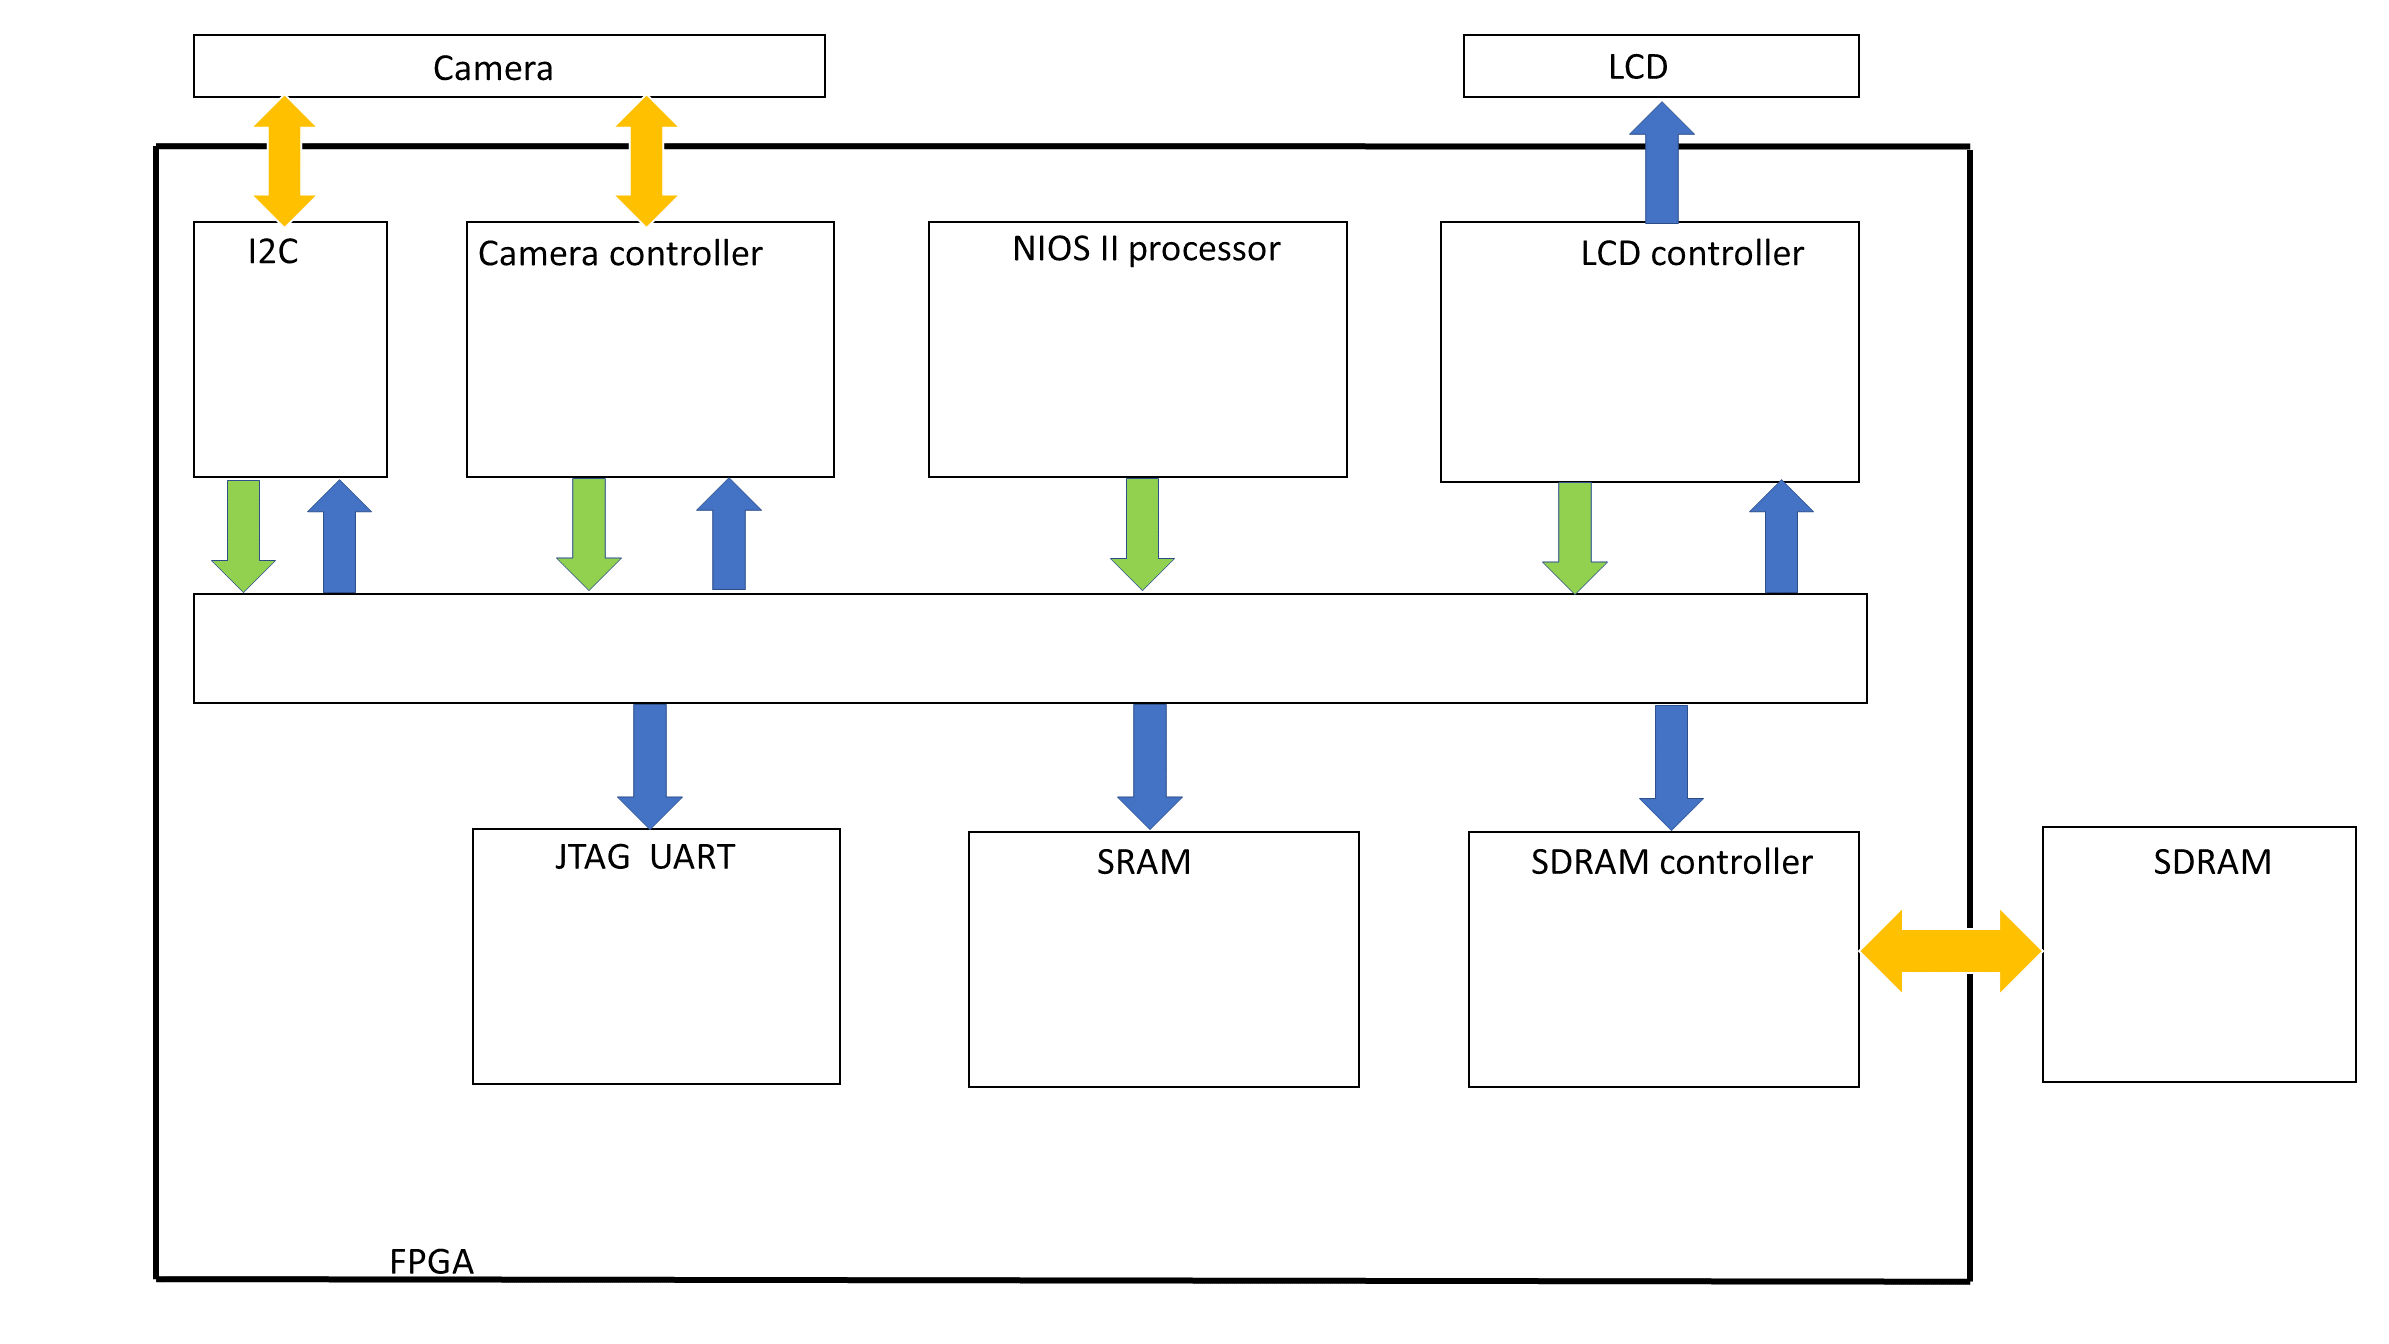
\includegraphics[scale=0.25]{full_system.png}
\caption{Full system architecture}
\label{fig:full_system}
\end{figure}

\subsection{Camera controller description}

Our camera component is divided into three main subcomponents.
The first one is an Avalon slave component, containing the readable/writable registers, which are accessible to the processor. These registers store configuration data for the other subcomponents.
The second subcomponent is the camera interface, which receives the camera sensor data, processes it to obtain desired RGB pixel values and finally forwards them into a FIFO buffer. 
A master Avalon component is the third block of our design. This block is responsible for reading pixel data from the FIFO and transferring it in a convenient format to the DRAM memory by using Avalon bus burst transfers.
To these three main parts of our system we include a PLL module to generate a clock signal \verb'XCLKIN' for the camera. The FIFO between camera interface and Avalon master component is dual-clock and allows to synchronize between the camera and the main clock domains.
Finally there is an I2C Avalon Slave which allows camera configuration by the NIOS-II processor.

\begin{figure}[H]
\centering
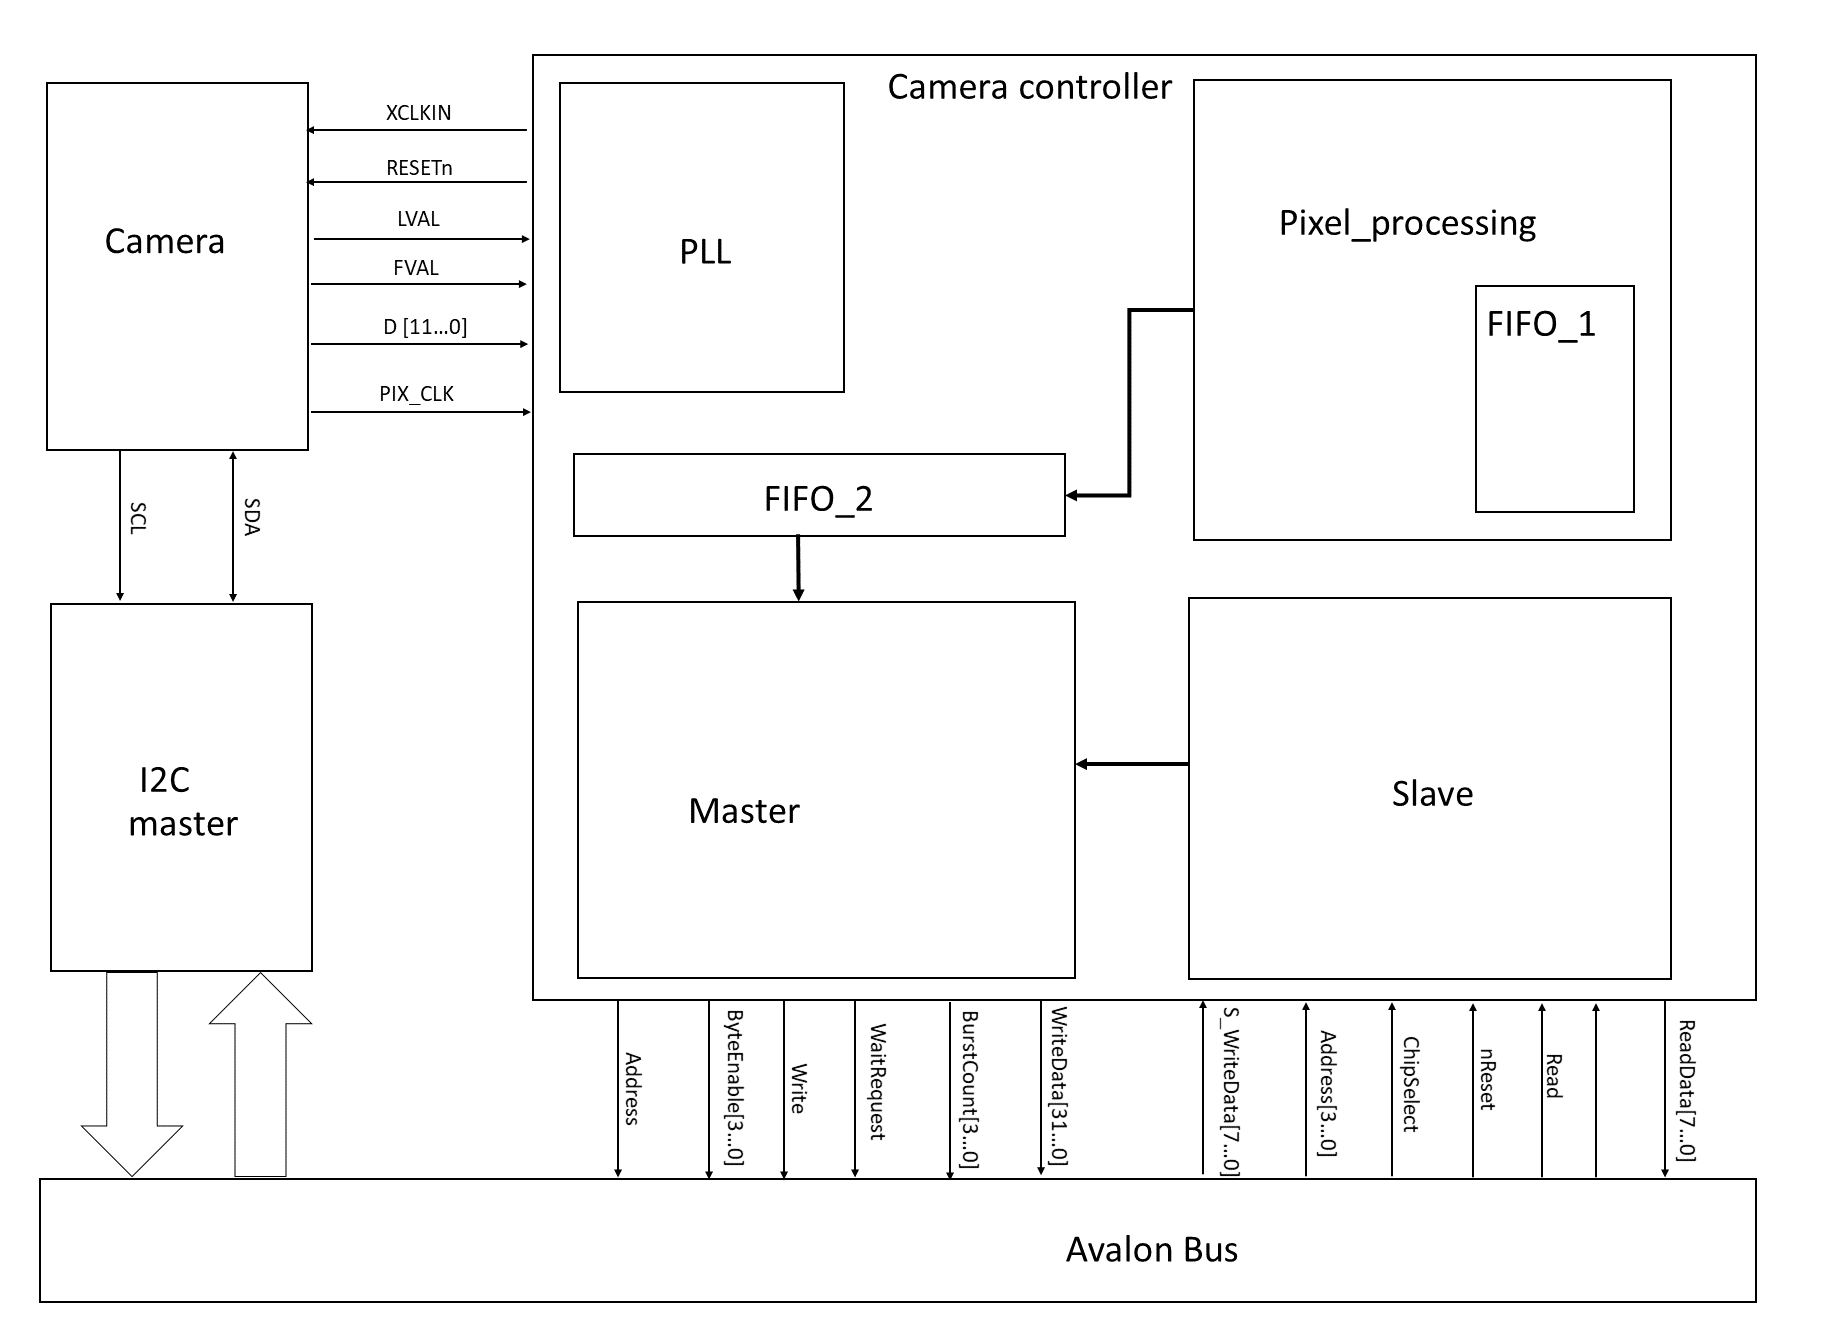
\includegraphics[width=\textwidth]{cam_ctrl_physical_arch.png}
\caption{Custom IP block diagram of the camera controller}
\label{fig:cam_ctrl_physical_arch}
\end{figure}


\section{Slave component}

The Avalon slave component consists of a set of configuration and control register accessible through an Avalon slave interface.
It also provides an interrupt line to notify the NIOS-II CPU of start and end of image reception. Furthermore it provides the image destination address to the master component and controls the internal enable signals and the camera reset line.
Figure \ref{fig:avalon_slave} shows the block diagram with the in- and out-going signals and the internal registers.

\begin{figure}[H]
\centering
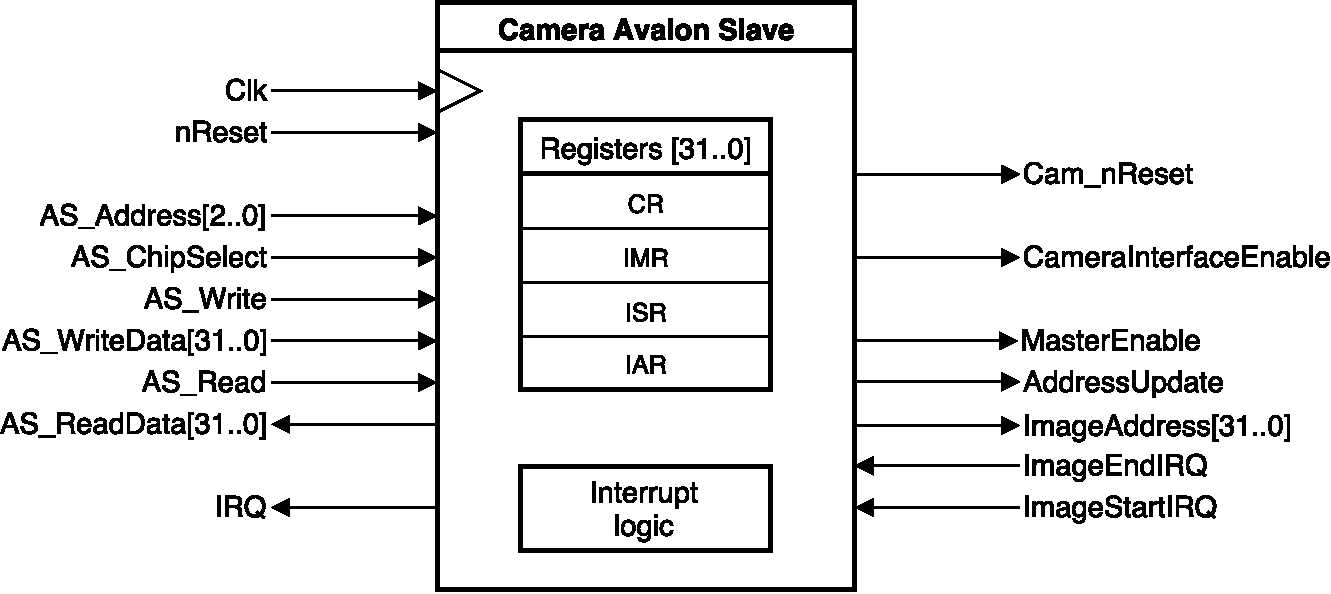
\includegraphics[width=\textwidth]{img/CameraAvalonSlave.pdf}
\caption{Camera Avalon slave block diagram}
\label{fig:avalon_slave}
\end{figure}

\subsection{Interrupts}
The camera controller provides an interrupt line with two configurable interrupt sources for start and end of image reception. The interrupts can be enabled in the Interrupt Mask Register (IMR). The camera interrupts can be used by the NIOS-II software to handle the image buffers.

\subsection{Register map}

\subsubsection{Control Register (CR)}
Address offset: 0x00 \\
Reset Value: 0x00000000 \\
[4mm]
\begin{bytefield}[endianness=big,bitwidth=2.5em]{16}
\bitheader[lsb=16]{16-31} \\
\bitbox{16}{Reserved}
\\
\bitheader{0-15} \\
\bitbox{14}{Reserved} &
\bitbox{1}{CE} &
\bitbox{1}{EN}
\end{bytefield}

\begin{registerdescription}
\item [Reserved] Bits 31:2, read only\\Reserved, read as 0
\item [CE] Bit 1, read/write\\Camera Enable. Controls the camera reset line.\\0: Camera is held in reset.\\1: Camera is enabled.
\item [EN] Bit 0, read/write\\Enable the Camera controller.\\0: Camera controller is disabled.\\1: Camera controller is enabled.
\end{registerdescription}

\subsubsection{Interrupt Mask Register (IMR)}
Address offset: 0x01 \\
Reset Value: 0x00000000 \\
[4mm]
\begin{bytefield}[endianness=big,bitwidth=2.5em]{16}
\bitheader[lsb=16]{16-31} \\
\bitbox{16}{Reserved}
\\
\bitheader{0-15} \\
\bitbox{14}{Reserved} &
\bitbox{1}{SIE} &
\bitbox{1}{EIE}
\end{bytefield}

\begin{registerdescription}
\item [Reserved] Bits 31:2, read only\\Reserved, read as 0
\item [SIE] Bit 1, read/write\\image reception Start Interrupt Enable.\\0: Interrupt is inhibited.\\1: Interrupt is generated when the bit SIF=1 in ISR register.
\item [EIE] Bit 0, read/write\\image reception End Interrupt Enable. \\0: Interrupt is inhibited.\\1: Interrupt is generated when the bit EIF=1 in ISR register.
\end{registerdescription}

\subsubsection{Interrupt Status Register (ISR)}
Address offset: 0x02 \\
Reset Value: 0x00000000 \\
[4mm]
\begin{bytefield}[endianness=big,bitwidth=2.5em]{16}
\bitheader[lsb=16]{16-31} \\
\bitbox{16}{Reserved}
\\
\bitheader{0-15} \\
\bitbox{14}{Reserved} &
\bitbox{1}{SIF} &
\bitbox{1}{EIF}
\end{bytefield}

\begin{registerdescription}
\item [Reserved] Bits 31:2, read only\\Reserved, read as 0
\item [SIF] Bit 1, read/write\\Start Interrupt Flag. Set by hardware when the reception of a new image frame starts. This bit must be cleared by software by writing a 1.
\item [EIF] Bit 0, read/write\\End Interrupt Flag. Set by hardware when the image data is completely written to memory. This bit must be cleared by software by writing a 1.
\end{registerdescription}

\subsubsection{Image Address Register (IAR)}
Address offset: 0x03 \\
Reset Value: 0x00000000 \\
[4mm]
\begin{bytefield}[endianness=big,bitwidth=2.5em]{16}
\bitheader[lsb=16]{16-31} \\
\bitbox{16}{IA[31:16]}
\\
\bitheader{0-15} \\
\bitbox{16}{IA[15:0]}
\end{bytefield}

\begin{registerdescription}
\item [IA] Bits 31:0, read/write\\Image Address. Destination address for the 320x240x2 = 153600 byte long image buffer. \\
Note: This register should be written only between image receptions to guarantee a correct address update. Ideally this is done in the "image reception end interrupt" ISR.
\end{registerdescription}


\section{Camera interface component}

The camera interface component acquires the 12-bit data from the camera sensors and transforms it to a 16-bit data for each pixel which are then forwarded into a FIFO buffer.

\subsection{Data reception}
The THDB-D5M camera provides a 12 bit data signal, a clock PIXCLK and control signals LVAL and FVAL for marking the valid image data window.
The image is transmitted line by line from top to bottom as shown in figure \ref{fig:image_transmission}.

\begin{figure}[H]
\centering
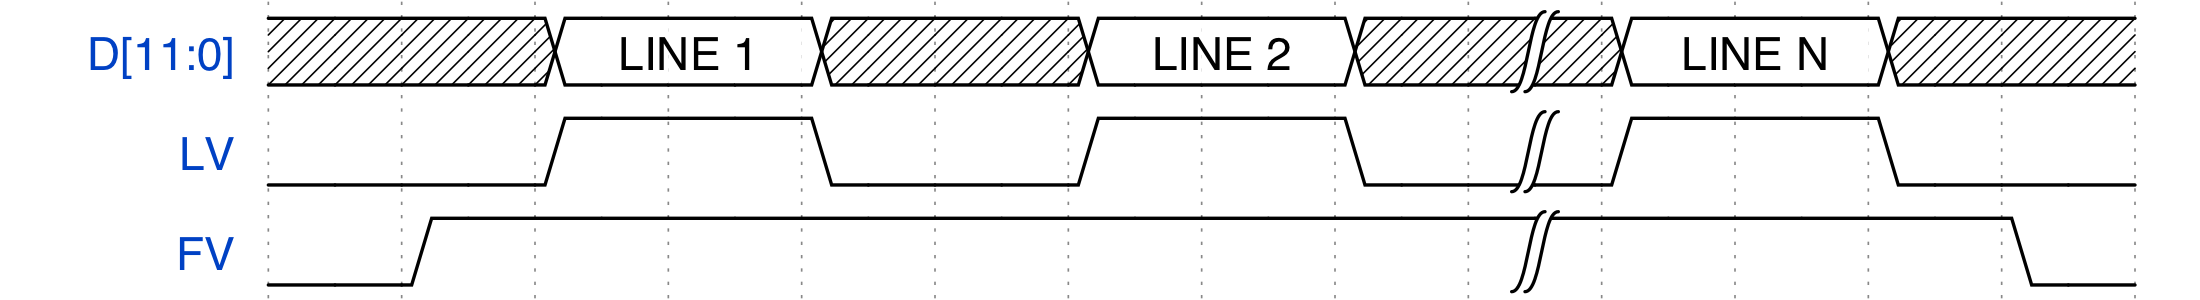
\includegraphics[width=\textwidth]{img/image_transmission.png}
\caption{Image transmission with LineValid and FrameValid signals.}
\label{fig:image_transmission}
\end{figure}

Each line contains the camera sensor data for the individual colors red, green and blue.
Figure figure \ref{fig:bayer_to_rgb} shows the bayer pattern composition for each pixel consisting of 4 color sensors: Red (R), green1 (G1), green2 (G2) and blue (B).
Pixels are separated over two lines: R and G1 on the first and G2 and B on the second.
Thus, to receive a line of pixels we have to receive 2 lines of color sensors as shown in figure \ref{fig:line_transmission}.

\begin{figure}[H]
\centering
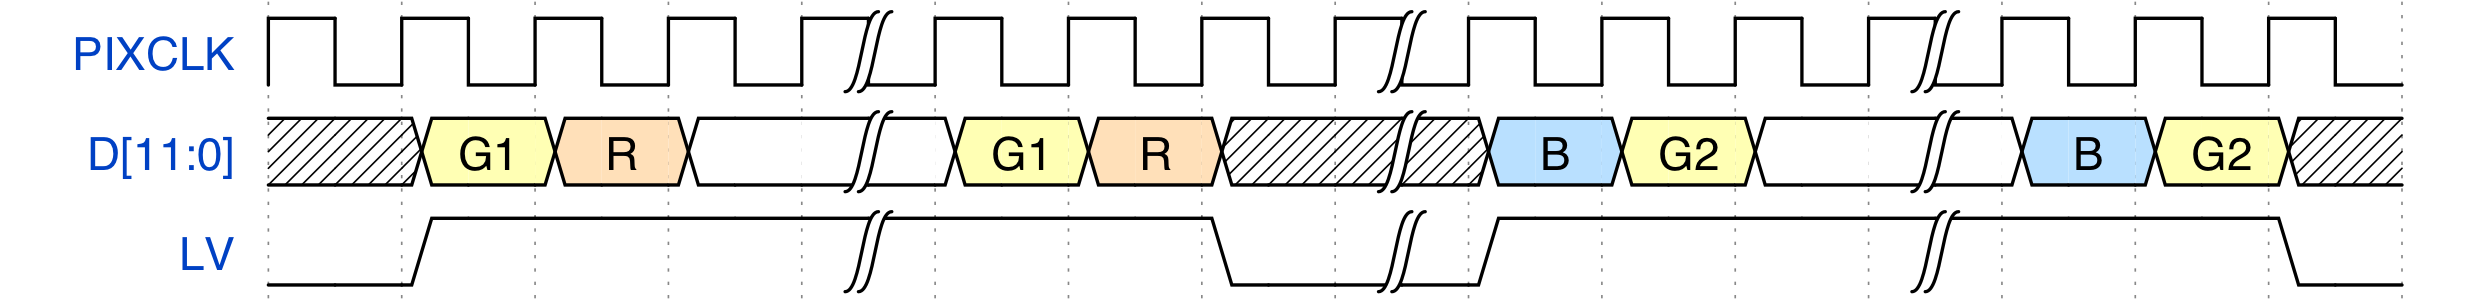
\includegraphics[width=\textwidth]{img/line_transmission.png}
\caption{Color sensor line transmission with bayer pattern ordering}
\label{fig:line_transmission}
\end{figure}

\subsection{Pixel data transformation}
To store the pixel values we decided for a compact 16bit format for one RGB pixel value consisting of 5bits red, 6bits green and 5bits blue, as illustrated in figure \ref{fig:bayer_to_rgb}.
Thus we only consider the 5 MSbits and simply discard the remaining LSbits from the sensor data.
By combining the two 5bit green values G1 and G2 we can simply add them together and obtain a 6bit value\footnote{Having a higher resolution for green makes sense, since the human eye is more sensitive in the green spectrum}.

\begin{figure}[H]
\centering
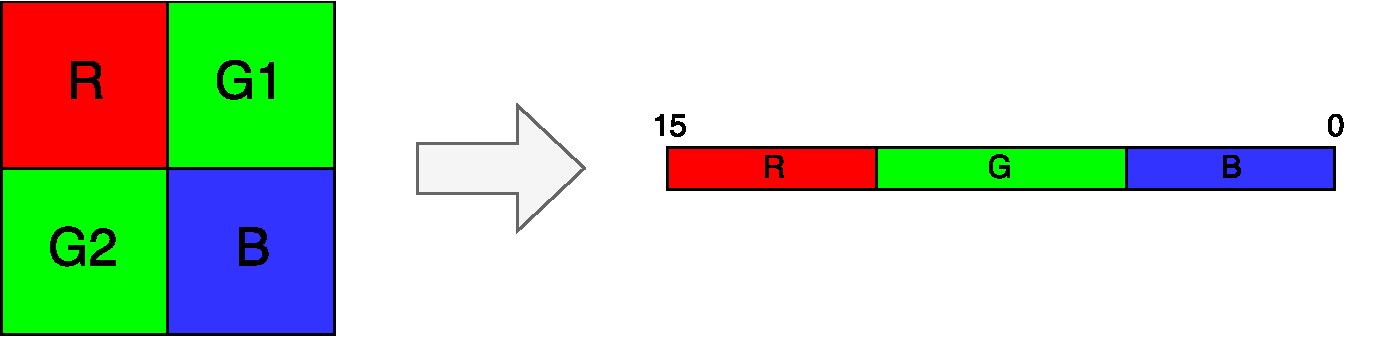
\includegraphics[width=0.7\textwidth]{img/CamBayerToRGB.pdf}
\caption{Bayer pattern to 16bit RGB (5bit,6bit,5bit) transformation.}
\label{fig:bayer_to_rgb}
\end{figure}

\subsection{Camera interface overview}
The camera interface component implements the process described above. It receives the camera data and control signals and outputs the transformed 16bit RGB pixel values to the pixel FIFO buffer.
The component consists of 3 main blocks: A FIFO to store a line of color sensor values, a processing unit to convert the bayer pattern to the RGB value and finally a finite state machine (FSM) that controls the two components and the output signals.
A diagram of the camera interface composition is shown in figure \ref{fig:camera_interface}.

\begin{figure}[H]
\centering
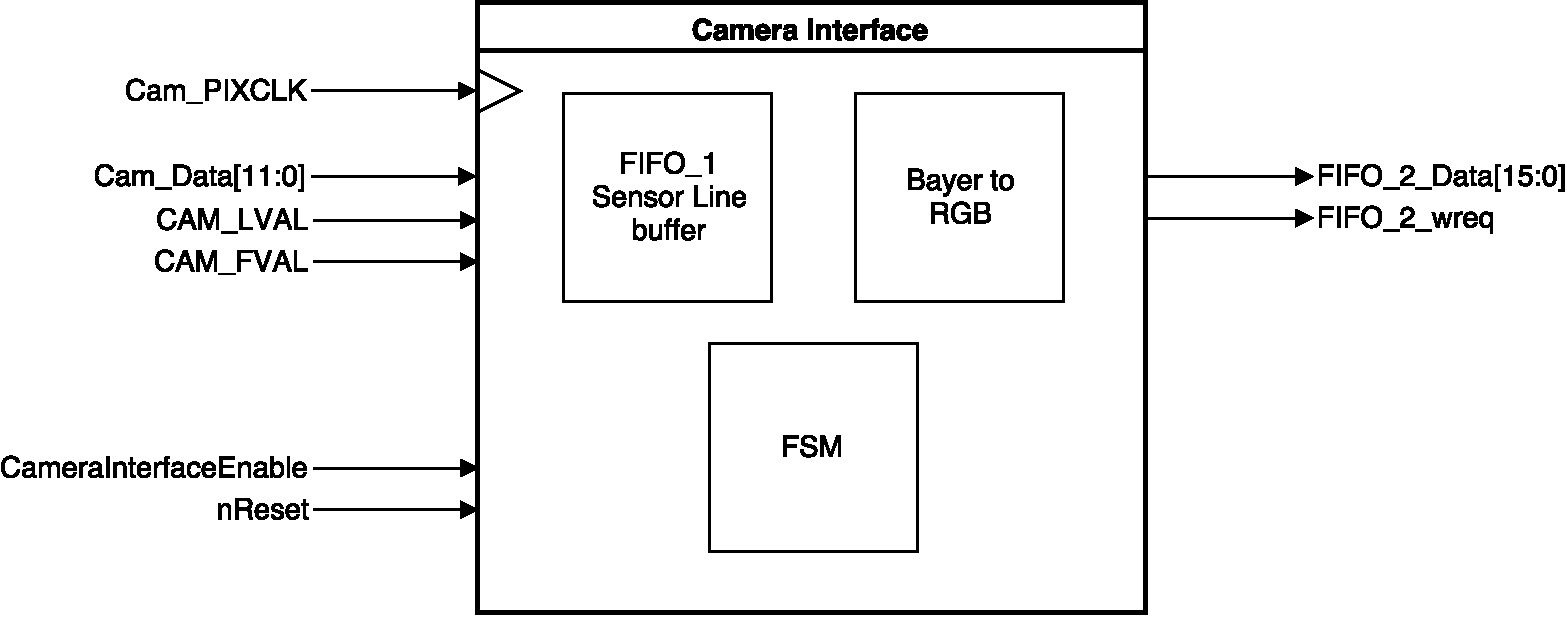
\includegraphics[width=\textwidth]{img/CameraInterface.pdf}
\caption{Camera interface block diagram}
\label{fig:camera_interface}
\end{figure}

\subsubsection{Bayer to RGB subcomponent}
Figure \ref{fig:bayer_phase} shows the order of the camera sensor data coming from the line FIFO and directly from the camera. For each pixel we identify two states: the state BLUE where colors blue and green1 are received and the state RED where colors red and green2 are receive.
\begin{figure}[H]
\centering
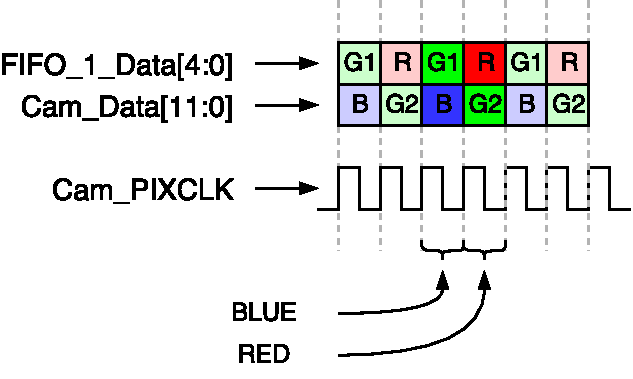
\includegraphics[width=0.6\textwidth]{img/BayerCombinePhase.pdf}
\caption{Bayer input signal order with indicated internal signals RED and BLUE}
\label{fig:bayer_phase}
\end{figure}

Figure \ref{fig:bayer_to_rgb_component} shows the process for transforming the bayer pattern to a RGB value. The states \verb'BLUE' and \verb'RED' are external signals provided by the camera interface FSM. During the first phase state \verb'BLUE' is active while state \verb'RED' is inactive. The colors green1 (G1) and blue (B) are buffered in 5bit registers. Next, the state \verb'BLUE' becomes inactive and state \verb'RED' becomes active. The buffered G1 and the incoming G2 are added to a 6bit green value. The result is combined with the buffered blue value and the incoming red value to a 16bit RGB signal which is provided as output of the "Bayer to RGB" subcomponent.
\begin{figure}[H]
\centering
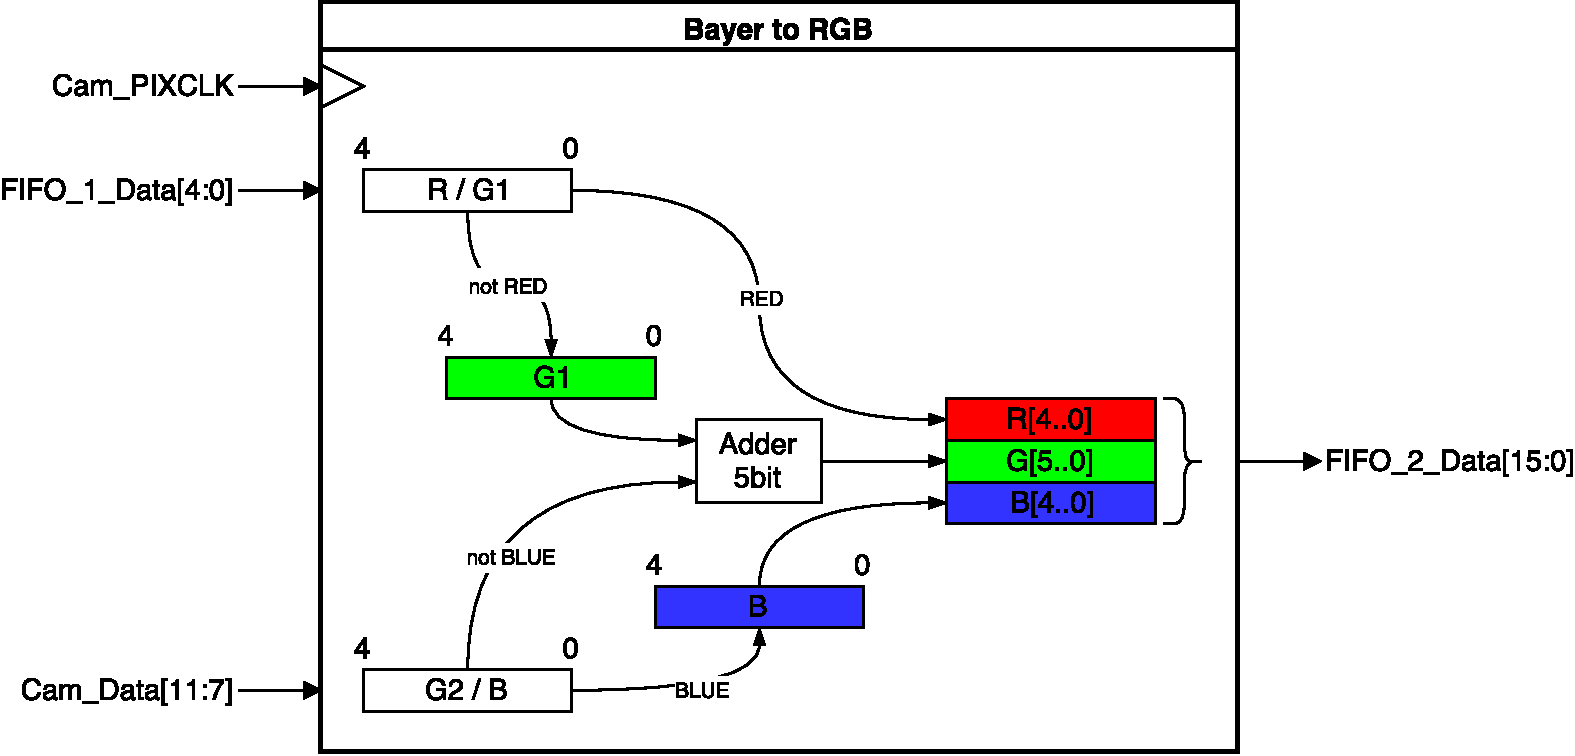
\includegraphics[width=\textwidth]{img/CameraInterfaceBayerToRGB.pdf}
\caption{Bayer to RGB transformation block diagram.}
\label{fig:bayer_to_rgb_component}
\end{figure}

\subsubsection{Sensor line FIFO}
The second subcomponent of the camera interface is a 2048x5-bit FIFO
\footnote{Quartus only allows for a 2048xNbit size. Actually only a 1280x5bit FIFO is needed.}
buffer which stores an entire line of color sensor data for later processing.

\subsubsection{Camera interface FSM}

We have three different FSM's working together in a hierarchical way, which are illustrated in figures \ref{fig:camera_interface_fsm}.

The lowest-level FSM has 3 states: \verb'IDLE', \verb'BLUE', \verb'RED'.
It defines which color is being read from the camera data lines and FIFO respectively. During state \verb'BLUE' the camera outputs the blue sensor value while the FIFO outputs green (G1) value. During state \verb'RED' the FIFO outputs the buffered red sensor value while the Camera outputs green (G2) value. This process is illustrated in figure \ref{fig:bayer_phase}.

The second FSM has 4 states: \verb'IDLE', \verb'PIXEL_BUFFER', \verb'PIXEL_OUTPUT' and \verb'PIXEL_SKIP'. In the state \verb'PIXEL_OUTPUT' the RGB pixel data is written into FIFO2. The state \verb'PIXEL_SKIP' results in the down sampling from 640 to 320 columns.

The last FSM at the highest hierarchical level has the following states:  \verb'IDLE', \verb'LINE_BUFFER', \verb'LINE_PROCESS', \verb'LINE_SKIP1' and \verb'LINE_SKIP2'. In the \verb'LINE_BUFFER' state a first line containing the red (R) and green (G1) sensor values is stored in FIFO1. Then, during the next \verb'LINE_PROCESS' state, the data from FIFO1 is read simultaneously with the incoming is data from the camera which is then transformed to a RGB pixel value by the "Bayer to RGB" component. The following two states \verb'LINE_SKIP1' and \verb'LINE_SKIP2' result in the down sampling from 480 to 240 lines.

%even sensor lines are stored into the FIFO, and then two consecutive lines are processed in the next state or ignored depending on a counter which handles the down-sampling of the image to 320x240 for the LCD. The way we intend to implement the down-sampling is to simply ignore 1 out of 2 lines of pixels by doing a normal computation on each line but deciding whether to store it into the second FIFO or not. 

\begin{figure}[H]
\centering
\hspace*{-0.1\textwidth}
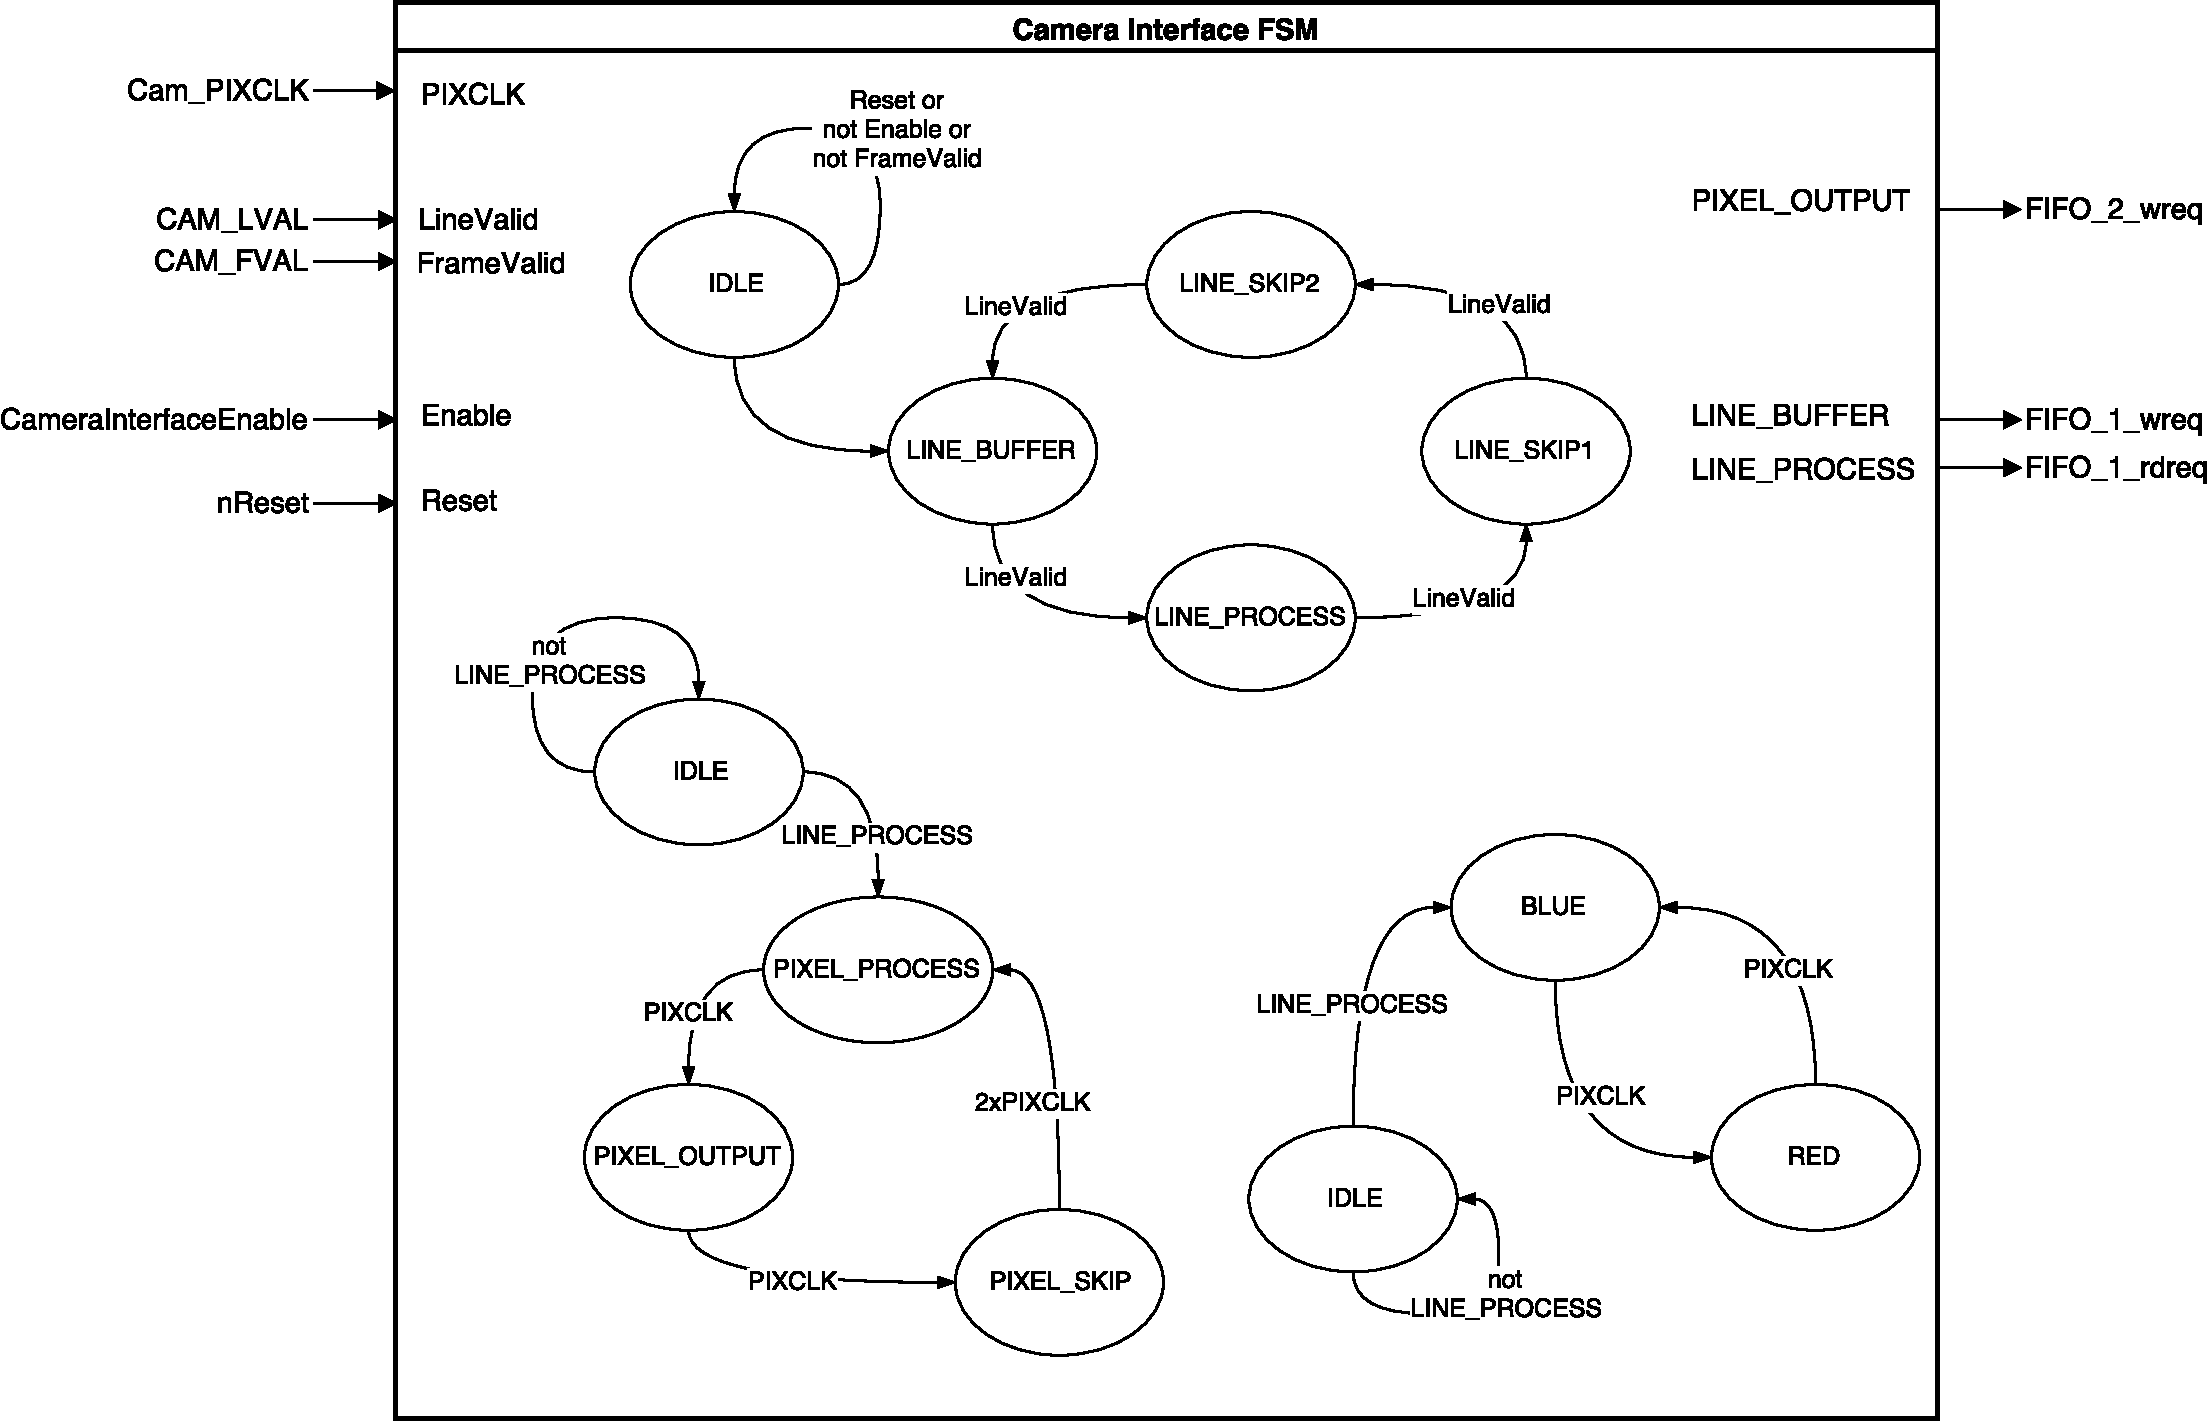
\includegraphics[width=1.2\textwidth]{img/CameraInterfaceFSM.pdf}
\caption{Finite state machine controlling the Camera interface}
\label{fig:camera_interface_fsm}
\end{figure}

Figure \ref{fig:camera_interface_signals} shows the desired waveform of the input and output signals. Only every second PIXCLK clock pulse a RGB pixel is calculated and only every second pixel is written in FIFO2 resulting in the horizontal down sampling from 640 to 320 pixel line width.

\begin{figure}[H]
\centering
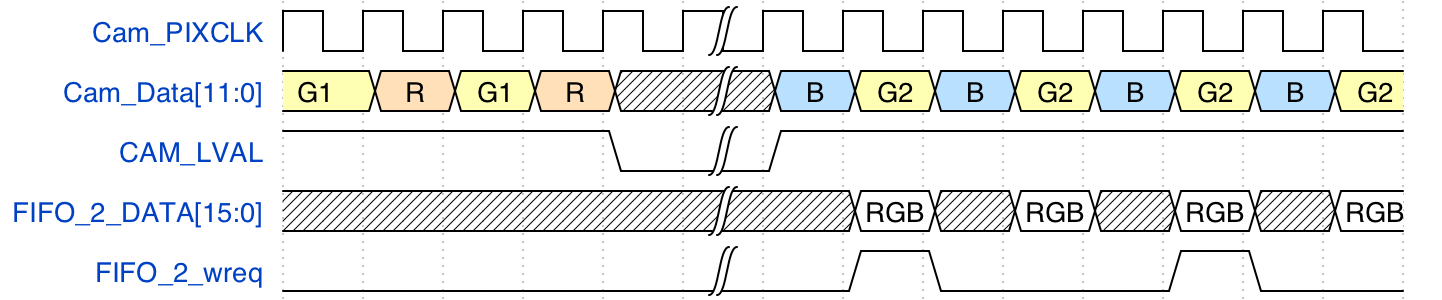
\includegraphics[width=\textwidth]{img/CameraInterfaceWaveDiagram.png}
\caption{Camera interface input and output signals wave diagram}
\label{fig:camera_interface_signals}
\end{figure}

%\begin{figure}[H]
%\centering
%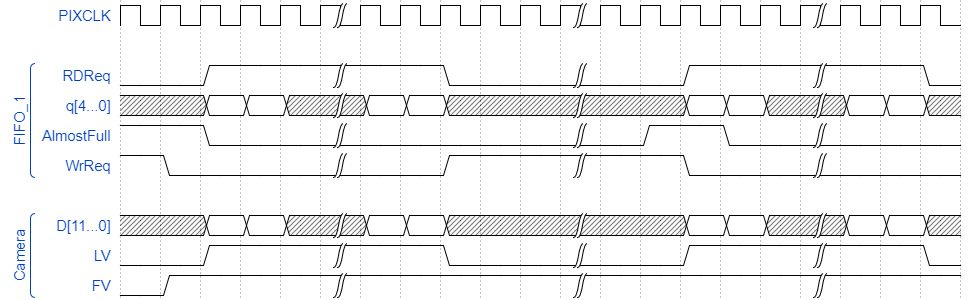
\includegraphics[width=0.8\textwidth]{timing2.PNG}
%\caption{Timing diagram of bayer combine FSM front-end signals}
%\label{fig:timingFSM}
%\end{figure}

\section{Master component}

\subsection{Description}
The master component is fully synchronous to the main clock domain. It reads data out of the 16x16-bit FIFO containing the desired format of the data to be stored in memory. Its main functionality is to transfer data through bursts to the SDRAM via an Avalon interface. We have defined the burst-length as 8 and on each burst count, a 32-bit signal is transferred to the off-chip memory. 16 pixels are thus sent to the memory in one burst. The FIFO is designed such that its total size matches the length of one burst to avoid inferring a counter in the control part of this block. 

\begin{figure}[H]
\centering
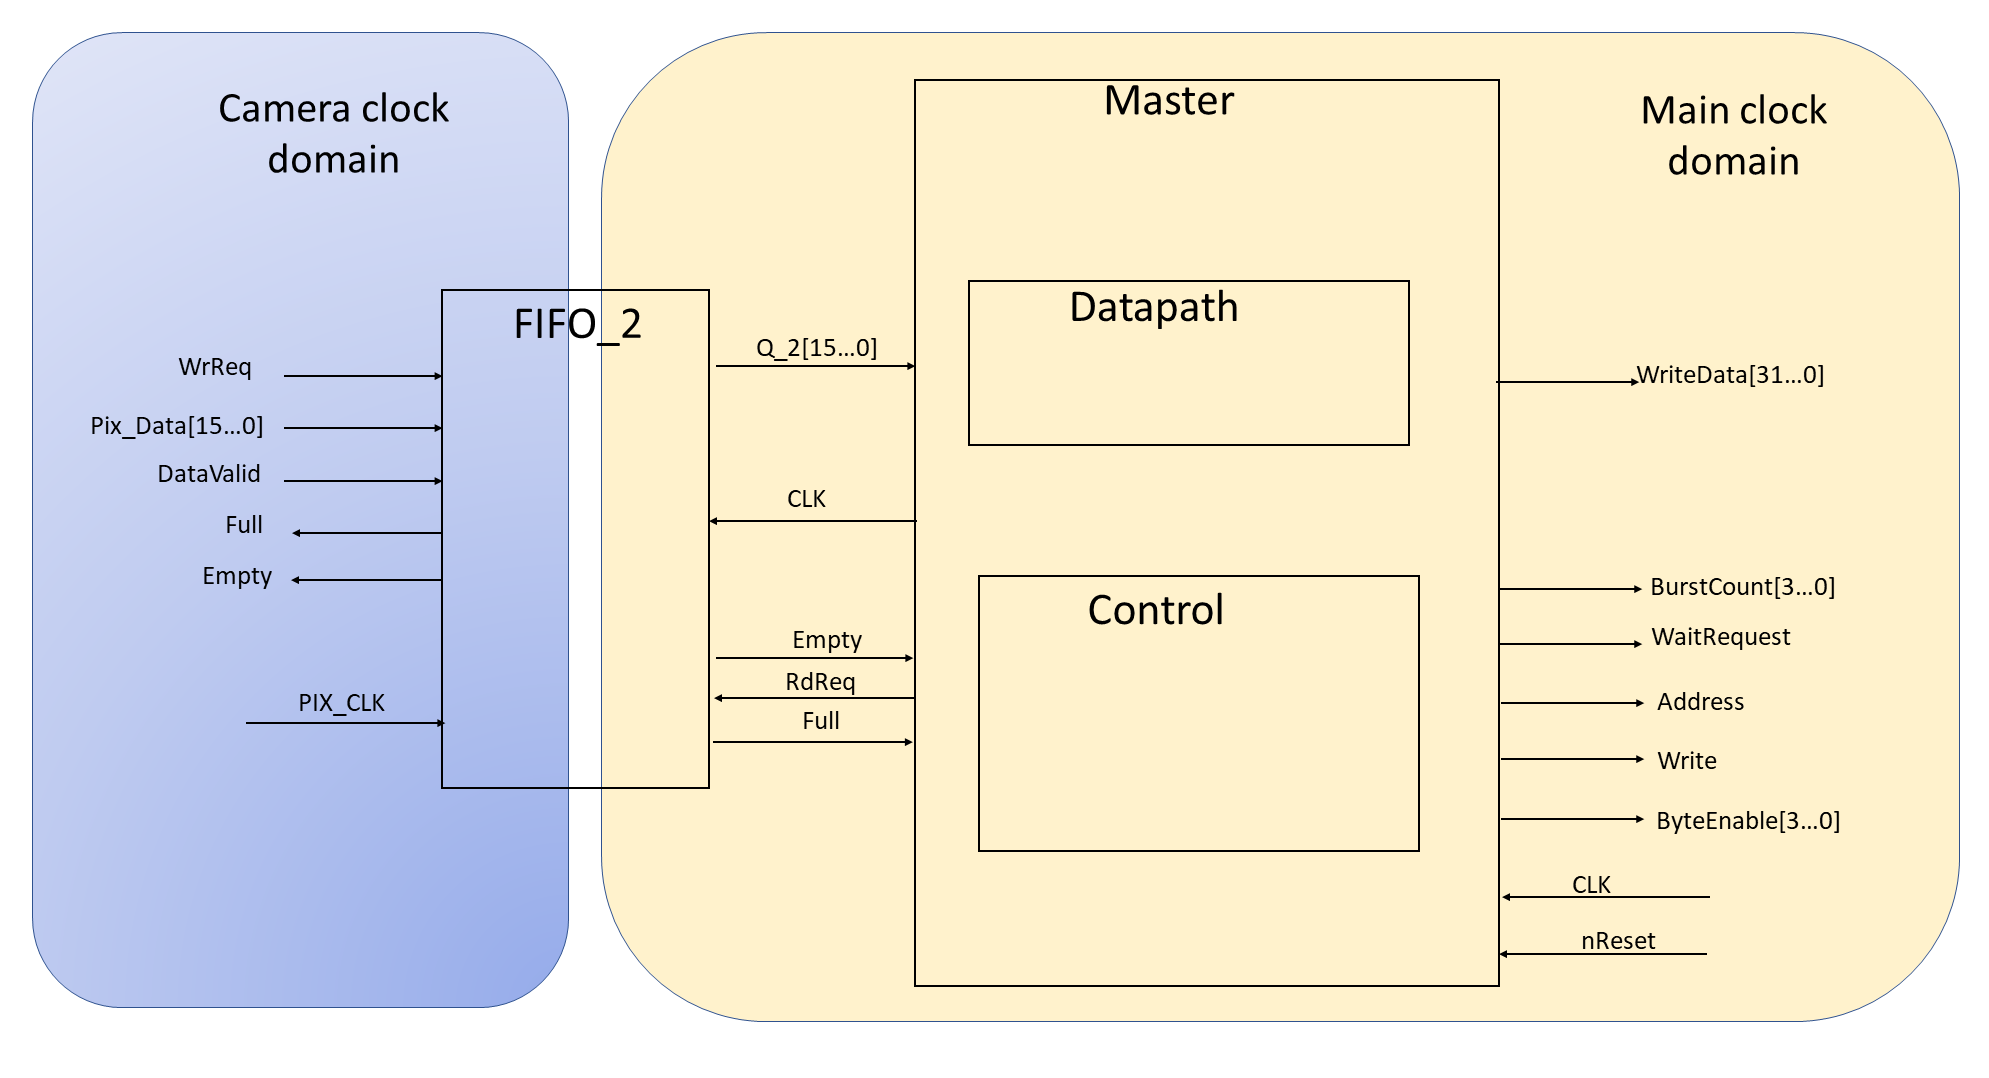
\includegraphics[scale=0.23]{master_block_diagram.png}
\caption{Architecture of Master component}
\label{fig:master_block_diagram}
\end{figure}

The input data being 16-bit sized (FIFO) and the output 32-bit sized (SDRAM), the master component needs to concatenate 2 consecutive inputs to build the output signal. This is done by the proposed datapath in Figure \ref{fig:master_datapath}.

\begin{figure}[H]
\centering
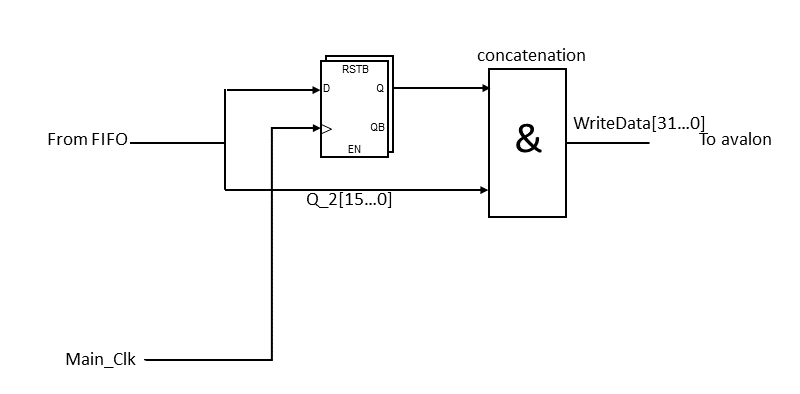
\includegraphics{master_datapath.png}
\caption{Proposed datapath architecture for the master component}
\label{fig:master_datapath}
\end{figure}

A simple 2-state FSM (Figure \ref{fig:master_control} is controlling the data flow and the interfacing between the master component, the FIFO and the Avalon bus. The timing of the interface signals of the FIFO with the master component are shown in Figure \ref{fig:timingMasterfront} and Figure \ref{fig:timingMasterAvalon} shows the timings of the Avalon interface signals.

\begin{figure}[H]
\centering
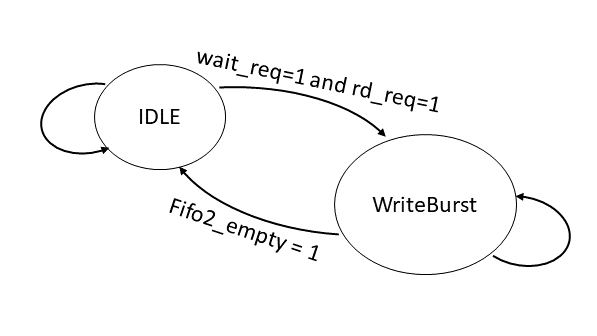
\includegraphics{master_control.png}
\caption{Proposed FSM for the master component control}
\label{fig:master_control}
\end{figure}

\begin{figure}[H]
\centering
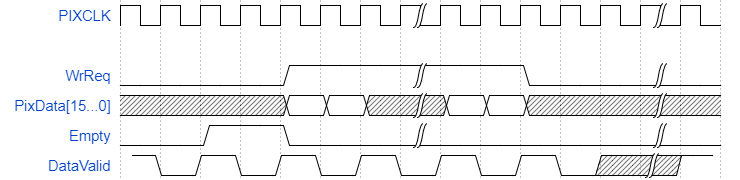
\includegraphics[scale=0.4]{timing3.PNG}
\caption{Timing diagram Master component front-end signals}
\label{fig:timingMasterfront}
\end{figure}

\begin{figure}[H]
\centering
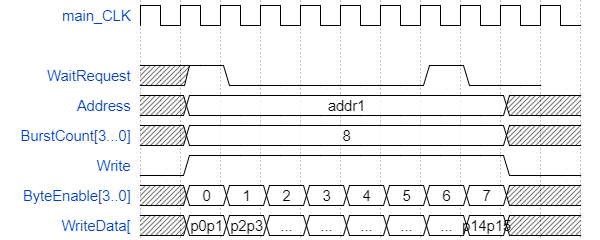
\includegraphics[scale=0.5]{timing4.PNG}
\caption{Timing diagram of Master Component/Avalon interface. WriteData is of size [31...0]}
\label{fig:timingMasterAvalon}
\end{figure}


\section{Data storage in memory}

The data of the camera is stored in the DRAM in 32 bit format, so 2 pixels are stored per memory 32-bit address. The readout direction of the camera is from right to left and from top to bottom, and the storage will have the same order, and the LCD has to be configured such that it writes the data back in this order which should be possible via software control in LCD slave registers. It should be done this way otherwise the data of the full image has to be stored fully in our custom camera component because the LCD default writing order is totally different (lines and columns are swapped and the order is from left to right). We cannot afford to store the full image because of on-chip memory limitations. 

\begin{figure}[H]
\centering
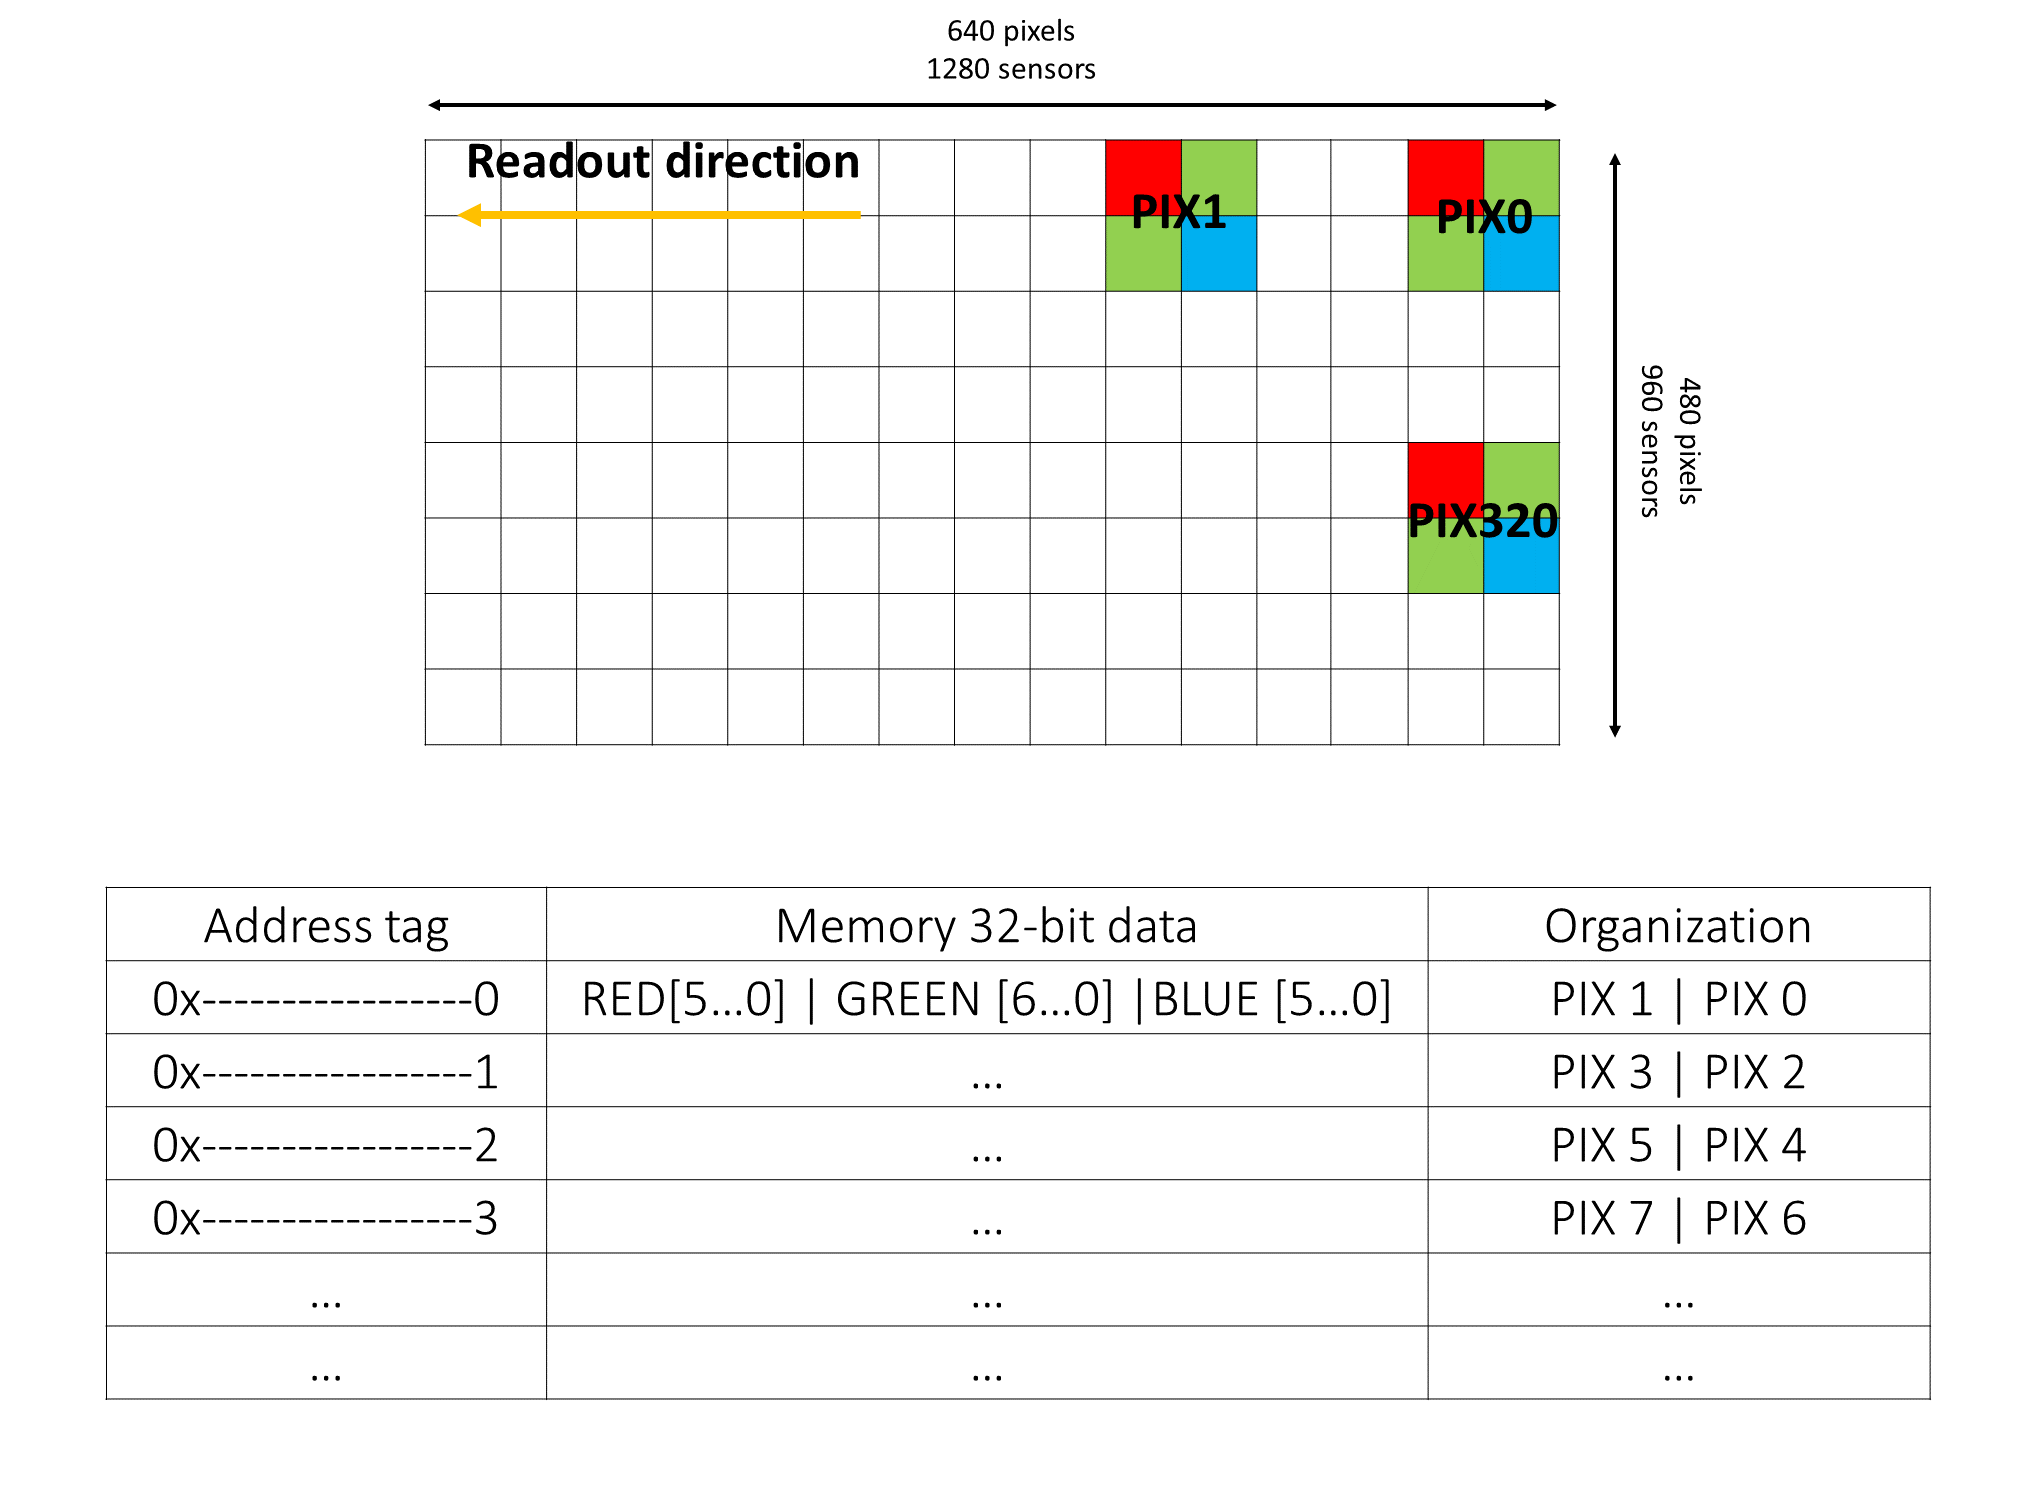
\includegraphics[scale=0.5]{memory_mapping.png}
\caption{Camera readout direction and SDRAM memory mapping}
\label{fig:memory_mapping}
\end{figure}

\section{Camera configuration}

\subsection{Clock}
Through a PLL component the FPGA system provides a clock to the camera throuth the XCLKIN line. The camera supports up to 96MHz clock frequency. We plan to configure the PLL to 50MHz and use this clock undivided as PIXCLK. This can be achieved by setting \verb'Divide_Pixel_Clock'=0 in \verb'Pixel Clock Control' register (bits 6:0 in R0x00A).

If a different clock is needed, the camera provides a configurable PLL.

%\subsection{Reset}
\subsection{I2C commands}

The camera is configured the usual way through I2C having read and write access to the 8bit address space with 2byte register size.

\paragraph{Register write}
A write access is done by addressing the camera through the I2C write address (0xBA) and then writing the 8bit register address followed by the two byte register data to be written. The register data is sent MSByte first.

\paragraph{Register read}
A read access happens in similar fashion by first addressing the camera through the I2C write address (0xBA) followed by sending the 8bit register address. Then the camera is addressed again using the I2C read address (0xBB) followed by reading the two byte register data.

\paragraph{Multiple read/write}
For both read and write access also multiple registers can be written at once using the address auto-increment. To do this, after the first register data transfer, the master can just continue reading or respectively writing data which will be read/written form the following registers.

\subsection{Register configuration}

We want to configure the camera to output an image of resolution 640x480 using binning sub sampling.
According to "Table 1.7 Standard Resolutions" in the TerasIC THDB-D5M Hardware specification we have to configure following registers:
\begin{itemize}
\item \verb'Row Size' = 1919 (R0x03)
\item \verb'Column Size' = 2559 (R0x04)
\item \verb'Shutter Width Lower' = 3 (R0x09)
\item \verb'Row_Bin' = 3 (R0x22 [5:4])
\item \verb'Row_Skip' = 3 (R0x22 [2:0])
\item \verb'Column_Bin' = 3 (R0x23 [5:4])
\item \verb'Column_Skip' = 3 (R0x23 [2:0])
\end{itemize}


After the register configuration we have to ensure that \verb'Chip Enable'=1 in \verb'Output Control' register (bit 2 in R0x07).


If for displaying reasons the image has to be mirrored, it is easiest to change the camera configuration to mirror row or column of the image.
This can be achieved by setting \verb'Mirror Row' or \verb'Mirror Column' in \verb'Read Mode 2' register (bits 15 or 14 in R0x20).

\subsection{Operation modes}
\subsubsection{Continuous}
For continuous mode we must clear the bit \verb'Snapshot' in register \verb'Read Mode 1' (bit 8 in R0x1E)

\subsubsection{Snapshot}
The camera allows also a snapshot mode where image capture can be triggered through the TRIGGER line or by setting \verb'Trigger'=1 in \verb'Reset' register (bit 2 in R0x0B).
For this the camera needs to be put into snapshot mode by setting \verb'Snapshot'=1 in register \verb'Read Mode 1' (bit 8 in R0x1E)

\subsubsection{Test pattern mode}
For testing our custom digital logic, the camera provides a \verb'Test_Pattern_Mode' which outputs a known color pattern, which facilitates debugging.

\end{document}
